\chapter{PK6 --- Nấu \& nhật ký}
\begin{figure}[H]\centering
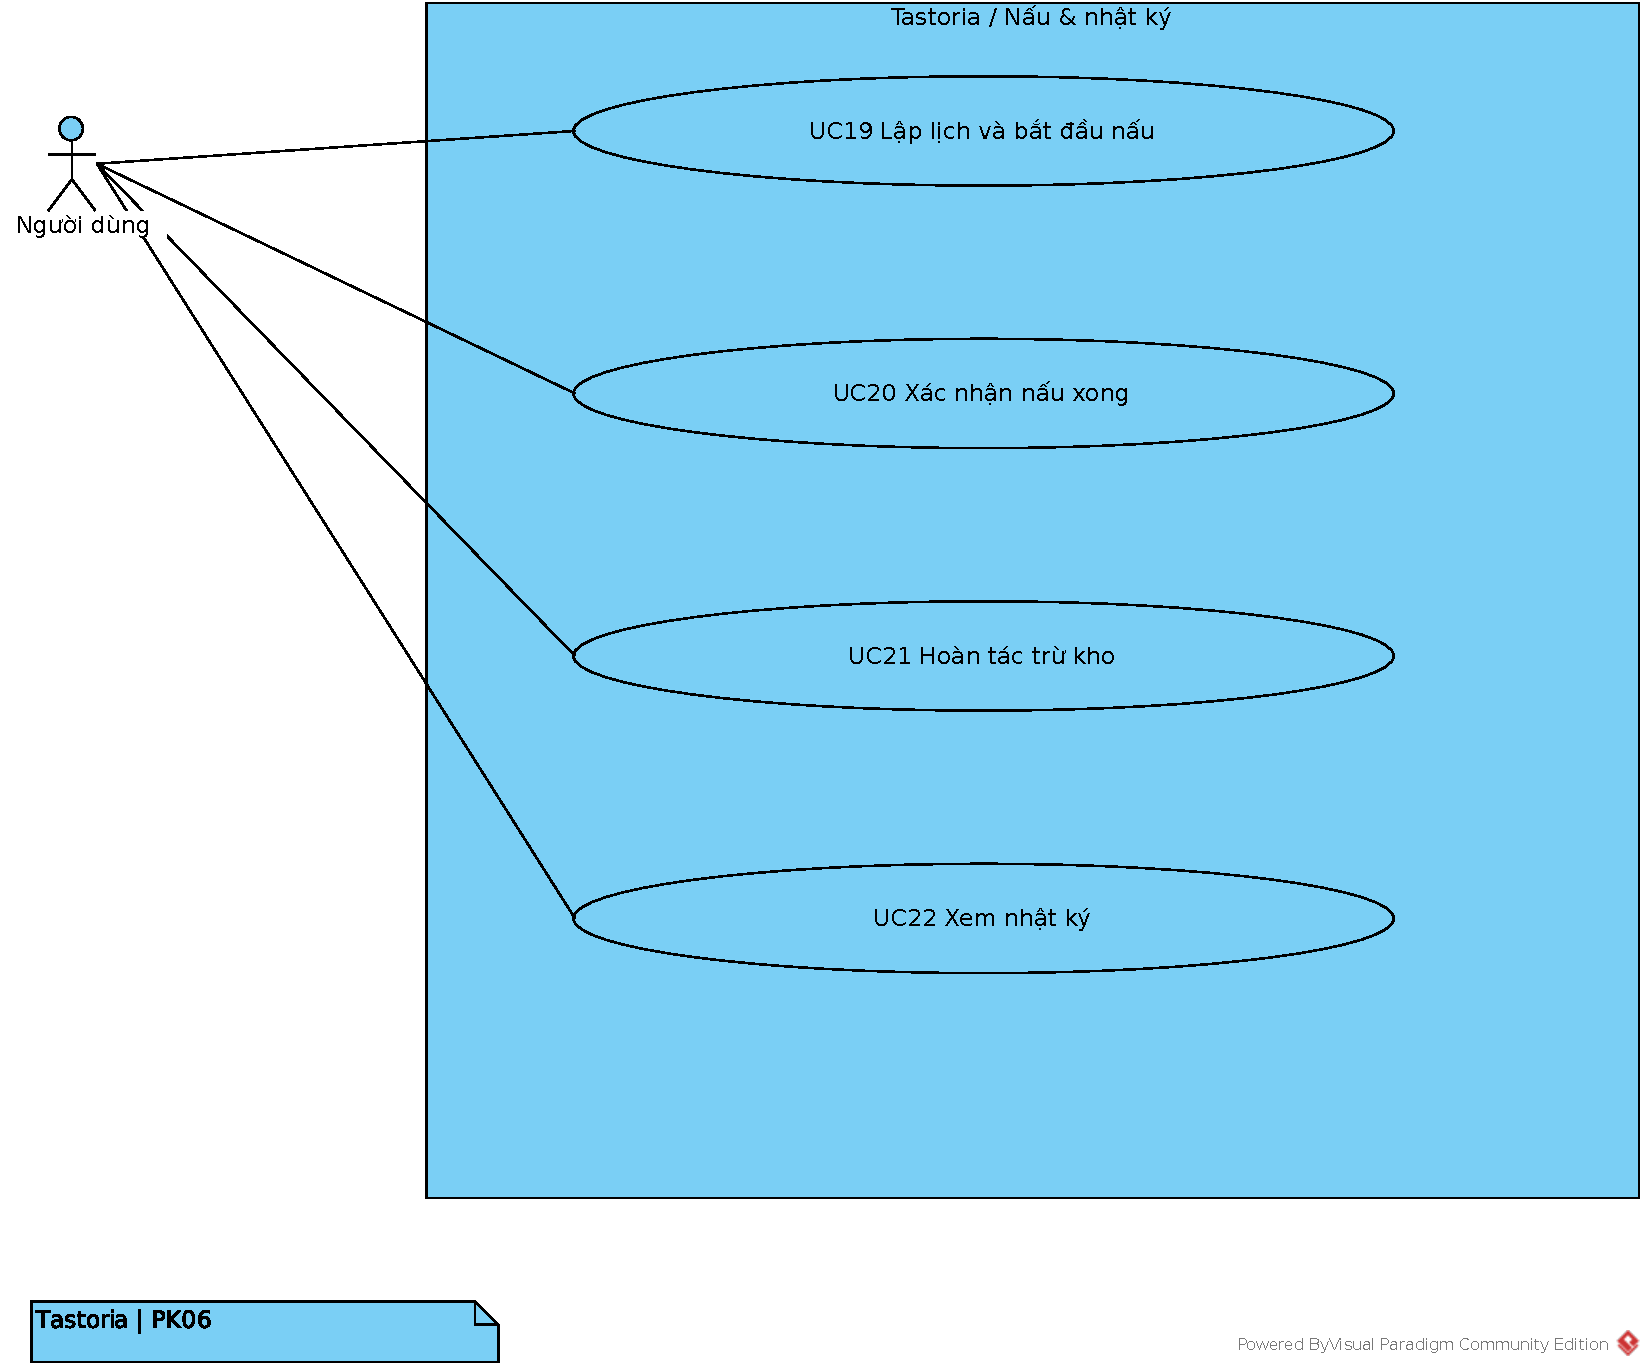
\includegraphics[width=0.96\linewidth,height=0.75\textheight,keepaspectratio]{assets/PK06.pdf}
\caption{PK06 --- Phân rã use case}\label{fig:Phu-luc-A-Use-Cases:6}
\end{figure}
\section{UC19 --- Nấu cả mâm}
\subsection{Mục tiêu trong ngữ cảnh}
Người dùng (A02) đã nhận một mâm cơm (UC15) và muốn nấu cả mâm cùng lúc. Hệ thống lập một lịch nấu song song cho các món đang hoạt động của mâm, sao cho một người nấu làm được, không vượt số họng bếp, mọi món xong gần giờ dọn mâm, rồi dẫn người dùng qua từng bước có đồng hồ đếm. Use case kết thúc khi người dùng chuyển sang "Nấu xong" (UC20) hoặc bỏ phiên nấu.

\subsection{Phạm vi và mức}
\begin{itemize}
\item Phạm vi: hệ thống Tastoria (app Android/\allowbreak{}web + backend), hộp đen.
\item Mức: mục tiêu người dùng (sea level).
\end{itemize}
\subsection{Tác nhân và bên liên quan (quyền lợi)}
{\footnotesize\setlength{\tabcolsep}{0pt}
\begin{longtable}{@{}L{7.850cm}@{\hspace{3mm}}L{7.850cm}@{}}
\caption{Tác nhân và bên liên quan (quyền lợi)}\\
\toprule
\textbf{Bên} & \textbf{Quyền lợi} \\
\midrule\endfirsthead
\multicolumn{2}{l}{\small\itshape Bảng \thetable{} (tiếp theo)}\\
\toprule
\textbf{Bên} & \textbf{Quyền lợi} \\
\midrule\endhead
\bottomrule\endfoot
A02 Người dùng (tác nhân chính) & Có lịch nấu làm theo được trên số họng bếp nhà mình, món xong nóng cùng lúc, món xào xong cuối; nấu tiếp được khi mất mạng. \\ \addlinespace[3pt]
Người ăn cùng (không tài khoản, qua A02) & Mâm được dọn đúng giờ đã hẹn. \\ \addlinespace[3pt]
Nhóm học máy (A06) & Sự kiện xem món chỉ được ghi khi người dùng đã đồng ý {\small\texttt{personalization}}; không có dữ liệu ngoài phạm vi đồng ý. \\ \addlinespace[3pt]
Nhóm phát triển & Lịch nấu tái lập được (ảnh chụp số họng bếp, lịch lưu theo phiên) để kiểm thử bất biến BR-\allowbreak{}COOK-\allowbreak{}01. \\ \addlinespace[3pt]
\end{longtable}}
\subsection{Tiền điều kiện}
\begin{enumerate}
\item A02 đã đăng nhập (access token hợp lệ, NFR-\allowbreak{}SEC-\allowbreak{}01).
\item Mâm {\small\texttt{meal\_\allowbreak{}\allowbreak{}plans}} thuộc A02 và có {\small\texttt{status = accepted}} (đã nhận ở UC15).
\item Mâm có 2 hoặc 3 {\small\texttt{meal\_\allowbreak{}\allowbreak{}plan\_\allowbreak{}\allowbreak{}items}} với {\small\texttt{status = active}} (BR-\allowbreak{}TRAY-\allowbreak{}01), mỗi món có ít nhất một dòng {\small\texttt{recipe\_\allowbreak{}\allowbreak{}steps}}.
\end{enumerate}
\subsection{Đảm bảo tối thiểu}
\begin{itemize}
\item Kho ({\small\texttt{pantry\_\allowbreak{}\allowbreak{}lots}}, {\small\texttt{pantry\_\allowbreak{}\allowbreak{}transactions}}) không bị thay đổi trong UC này; trừ kho chỉ xảy ra ở UC20.
\item Không có hai phiên {\small\texttt{cook\_\allowbreak{}\allowbreak{}sessions}} ở {\small\texttt{in\_\allowbreak{}\allowbreak{}progress}} cho cùng một mâm.
\item Gửi lại cùng {\small\texttt{Idempotency-\allowbreak{}Key}} không tạo phiên thứ hai.
\item Không ghi {\small\texttt{interactions}} khi A02 chưa đồng ý {\small\texttt{personalization}} (BR-\allowbreak{}CONSENT-\allowbreak{}03).
\end{itemize}
\subsection{Đảm bảo khi thành công}
\begin{itemize}
\item Có đúng một {\small\texttt{cook\_\allowbreak{}\allowbreak{}sessions}} ở {\small\texttt{in\_\allowbreak{}\allowbreak{}progress}} cho mâm, với {\small\texttt{serve\_\allowbreak{}\allowbreak{}at}}, {\small\texttt{burners}} (ảnh chụp số họng bếp lúc tạo), {\small\texttt{started\_\allowbreak{}\allowbreak{}at}}.
\item {\small\texttt{cook\_\allowbreak{}\allowbreak{}schedule\_\allowbreak{}\allowbreak{}entries}} chứa mọi bước của mọi món đang hoạt động, mỗi bước một khoảng [{\small\texttt{start\_\allowbreak{}\allowbreak{}offset\_\allowbreak{}\allowbreak{}s}}, {\small\texttt{end\_\allowbreak{}\allowbreak{}offset\_\allowbreak{}\allowbreak{}s}}) tính từ {\small\texttt{started\_\allowbreak{}\allowbreak{}at}}, thoả BR-\allowbreak{}COOK-\allowbreak{}01 và BR-\allowbreak{}TRAY-\allowbreak{}05.
\item App có bản sao lịch và các bước món (từ {\small\texttt{GET /\allowbreak{}\allowbreak{}catalog/\allowbreak{}\allowbreak{}snapshot}}) trong SQLite để chạy tiếp khi mất mạng.
\end{itemize}
\subsection{Kích hoạt}
A02 chạm "Nấu cả mâm" trên màn hình Mâm cơm hôm nay của một mâm đã nhận.

\subsection{Kịch bản chính}
Kịch bản viết ở mức tác nhân \ensuremath{\leftrightarrow} hệ thống (hộp đen). Lời gọi giữa module {\small\texttt{cooking}}, {\small\texttt{meal}}, {\small\texttt{profile}}, {\small\texttt{catalog}} và cách dựng bài toán CP-\allowbreak{}SAT (ADR 0009) là thiết kế, không phải yêu cầu.

\begin{enumerate}
\item A02 chạm "Nấu cả mâm", chọn giờ dọn mâm (mặc định: sớm nhất có thể).
\item App sinh một {\small\texttt{Idempotency-\allowbreak{}Key}} (UUID) và gửi {\small\texttt{POST /\allowbreak{}\allowbreak{}cook-\allowbreak{}sessions}} với {\small\texttt{meal\_\allowbreak{}\allowbreak{}plan\_\allowbreak{}\allowbreak{}id}}, {\small\texttt{serve\_\allowbreak{}\allowbreak{}at}}.
\item Hệ thống kiểm khoá lũy đẳng; khoá mới thì đi tiếp.
\item Hệ thống kiểm mâm thuộc A02 và đang {\small\texttt{accepted}}, lấy các món {\small\texttt{active}}, thời gian tối đa và số người của mâm.
\item Hệ thống kiểm mâm chưa có phiên nấu {\small\texttt{in\_\allowbreak{}\allowbreak{}progress}} nào khác.
\item Hệ thống lấy số họng bếp của A02.
\item Hệ thống lấy các bước (thứ tự, chủ động/\allowbreak{}thụ động, số phút, có chiếm bếp) và cách nấu của đúng bản món mà mâm trỏ tới (BR-\allowbreak{}CATALOG-\allowbreak{}01).
\item Hệ thống lập lịch nấu thoả BR-\allowbreak{}COOK-\allowbreak{}01 (không hai bước chủ động cùng lúc; số bước chiếm bếp đồng thời \ensuremath{\leq} số họng bếp; bước trong món theo thứ tự; mọi món xong trong cửa sổ 5 phút trước giờ dọn; món xào xong cuối) với makespan nhỏ nhất.
\item Hệ thống kiểm makespan \ensuremath{\leq} thời gian tối đa của mâm (BR-\allowbreak{}TRAY-\allowbreak{}05).
\item Hệ thống lưu phiên nấu {\small\texttt{in\_\allowbreak{}\allowbreak{}progress}} cùng lịch nấu và ghi nhớ phản hồi theo khoá lũy đẳng trong một giao dịch.
\item Hệ thống trả {\small\texttt{201}} kèm lịch nấu (theo bước: món, mô tả, giờ bắt đầu/\allowbreak{}kết thúc, cờ chủ động/\allowbreak{}chiếm bếp) và makespan.
\item App gọi {\small\texttt{GET /\allowbreak{}\allowbreak{}catalog/\allowbreak{}\allowbreak{}snapshot}} nếu bản catalog trong SQLite cũ hơn bản server, lưu lịch vào SQLite, bật keep-\allowbreak{}awake.
\item App hiện màn hình Nấu cả mâm: dòng thời gian theo món, bước hiện tại, đồng hồ đếm ngược, báo trước bước kế tiếp; A02 làm theo, chạm "Xong bước" hoặc để đồng hồ tự chuyển với bước thụ động.
\item Nếu A02 đã đồng ý {\small\texttt{personalization}}, app gửi {\small\texttt{POST /\allowbreak{}\allowbreak{}events}} (sự kiện {\small\texttt{viewed}}, có {\small\texttt{event\_\allowbreak{}\allowbreak{}id}}) khi A02 mở chi tiết một món; hệ thống chỉ ghi tương tác khi có đồng ý.
\item Khi bước cuối của lịch xong, app chuyển sang màn hình Nấu xong; use case kết thúc và UC20 bắt đầu.
\end{enumerate}
\subsection{Mở rộng}
\begin{itemize}
\item \textbf{1a. Giờ dọn mâm sớm hơn thời điểm hiện tại + makespan nhỏ nhất:} ở bước 8, hệ thống đặt {\small\texttt{serve\_\allowbreak{}\allowbreak{}at}} = {\small\texttt{now()}} + makespan nhỏ nhất, trả lịch kèm cờ {\small\texttt{serve\_\allowbreak{}\allowbreak{}at\_\allowbreak{}\allowbreak{}adjusted = true}}; app hiện "Sớm nhất dọn mâm lúc hh:mm".
\item \textbf{2a. Mất mạng khi gửi {\small\texttt{POST /\allowbreak{}\allowbreak{}cook-\allowbreak{}sessions}}:} app giữ nguyên {\small\texttt{Idempotency-\allowbreak{}Key}}, gửi lại khi có mạng (tối đa theo chính sách thử lại của client); app không cho bắt đầu đồng hồ khi chưa có lịch từ server.
\item \textbf{3a. Gửi lại cùng {\small\texttt{Idempotency-\allowbreak{}Key}} và cùng nội dung:} hệ thống trả nguyên văn phản hồi đã lưu (cùng mã trạng thái, cùng {\small\texttt{cook\_\allowbreak{}\allowbreak{}session\_\allowbreak{}\allowbreak{}id}}); không tạo phiên mới.
\item \textbf{3b. Cùng {\small\texttt{Idempotency-\allowbreak{}Key}} nhưng nội dung khác:} hệ thống trả {\small\texttt{422}} {\small\texttt{application/\allowbreak{}\allowbreak{}problem+json}}, {\small\texttt{code = idempotency\_\allowbreak{}\allowbreak{}key\_\allowbreak{}\allowbreak{}reused}}; không ghi gì.
\item \textbf{4a. Mâm không tồn tại hoặc thuộc người khác:} trả {\small\texttt{404}} (chống BOLA); không tiết lộ mâm có tồn tại hay không.
\item \textbf{4b. Mâm ở {\small\texttt{proposed}}:} trả {\small\texttt{409}}, {\small\texttt{code = meal\_\allowbreak{}\allowbreak{}plan\_\allowbreak{}\allowbreak{}not\_\allowbreak{}\allowbreak{}accepted}}; app đưa A02 về bước nhận mâm của UC15.
\item \textbf{4c. Mâm ở {\small\texttt{cooked}}, {\small\texttt{abandoned}} hoặc {\small\texttt{expired}}:} trả {\small\texttt{409}}, {\small\texttt{code = meal\_\allowbreak{}\allowbreak{}plan\_\allowbreak{}\allowbreak{}not\_\allowbreak{}\allowbreak{}cookable}}.
\item \textbf{5a. Đã có phiên {\small\texttt{in\_\allowbreak{}\allowbreak{}progress}} của mâm:} trả {\small\texttt{409}}, {\small\texttt{code = cook\_\allowbreak{}\allowbreak{}session\_\allowbreak{}\allowbreak{}in\_\allowbreak{}\allowbreak{}progress}}, kèm {\small\texttt{cook\_\allowbreak{}\allowbreak{}session\_\allowbreak{}\allowbreak{}id}} đang chạy; app mở lại phiên đó bằng {\small\texttt{GET /\allowbreak{}\allowbreak{}cook-\allowbreak{}sessions/\allowbreak{}\allowbreak{}\{id\}}}.
\item \textbf{7a. Một món không có bước nào (lỗi dữ liệu kho món):} trả {\small\texttt{422}}, {\small\texttt{code = recipe\_\allowbreak{}\allowbreak{}without\_\allowbreak{}\allowbreak{}steps}}, ghi log lỗi kèm {\small\texttt{recipe\_\allowbreak{}\allowbreak{}id}} để A05 sửa ở UC25.
\item \textbf{8a. Bộ giải không tìm được lời giải trong giới hạn thời gian:} hệ thống dùng lịch dự phòng xếp tuần tự từng món (vẫn thoả NoOverlap, Cumulative và thứ tự bước), trả kèm {\small\texttt{solver\_\allowbreak{}\allowbreak{}status = fallback}}.
\item \textbf{9a. Makespan > {\small\texttt{max\_\allowbreak{}\allowbreak{}minutes}} (không khả thi về thời gian):} hệ thống vẫn trả lịch tốt nhất kèm {\small\texttt{over\_\allowbreak{}\allowbreak{}time\_\allowbreak{}\allowbreak{}minutes}}; app hỏi A02 "Lịch cần x phút, quá y phút đã chọn. Vẫn nấu?". Phản hồi này trả {\small\texttt{200}} và không tạo phiên. Đồng ý thì app gửi lại {\small\texttt{POST /\allowbreak{}\allowbreak{}cook-\allowbreak{}sessions}} có cờ xác nhận với một {\small\texttt{Idempotency-\allowbreak{}Key}} mới (thân khác nên không dùng lại khoá cũ) và hệ thống đi tiếp bước 10; không thì không tạo phiên, A02 quay lại UC15 (đổi món ở UC16).
\item \textbf{10a. Lỗi cơ sở dữ liệu khi ghi:} giao dịch rollback, không lưu khoá lũy đẳng; trả {\small\texttt{503}}, {\small\texttt{code = temporarily\_\allowbreak{}\allowbreak{}unavailable}}; app thử lại với cùng {\small\texttt{Idempotency-\allowbreak{}Key}}.
\item \textbf{13a. Mất mạng trong lúc nấu:} app chạy tiếp hoàn toàn từ lịch và bước món trong SQLite; không cần gọi server cho tới UC20.
\item \textbf{13b. App bị đóng hoặc máy khởi động lại:} khi mở lại, app đọc phiên trong SQLite, gọi {\small\texttt{GET /\allowbreak{}\allowbreak{}cook-\allowbreak{}sessions/\allowbreak{}\allowbreak{}\{id\}}} nếu có mạng để đồng bộ trạng thái, tính lại bước hiện tại theo {\small\texttt{started\_\allowbreak{}\allowbreak{}at}} và đồng hồ máy.
\item \textbf{13c. A02 bỏ nấu giữa chừng:} A02 chạm "Bỏ phiên nấu"; app gửi {\small\texttt{POST /\allowbreak{}\allowbreak{}cook-\allowbreak{}sessions/\allowbreak{}\allowbreak{}\{id\}/\allowbreak{}\allowbreak{}abandon}}; hệ thống chuyển phiên {\small\texttt{in\_\allowbreak{}\allowbreak{}progress \ensuremath{\rightarrow} abandoned}}; kho không đổi; mâm giữ {\small\texttt{accepted}}. Gửi lại khi phiên đã {\small\texttt{abandoned}} trả {\small\texttt{200}} với trạng thái hiện tại.
\item \textbf{13d. Bỏ phiên khi phiên đã {\small\texttt{completed}} hoặc {\small\texttt{reverted}}:} trả {\small\texttt{409}}, {\small\texttt{code = cook\_\allowbreak{}\allowbreak{}session\_\allowbreak{}\allowbreak{}not\_\allowbreak{}\allowbreak{}in\_\allowbreak{}\allowbreak{}progress}}.
\item \textbf{13e. A02 muốn xem công thức đầy đủ của một món:} app gọi {\small\texttt{GET /\allowbreak{}\allowbreak{}recipes/\allowbreak{}\allowbreak{}\{id\}}} (hoặc đọc SQLite khi mất mạng).
\item \textbf{14a. A02 chưa đồng ý hoặc đã rút đồng ý {\small\texttt{personalization}}:} app không gửi sự kiện; nếu sự kiện vẫn tới server, hệ thống bỏ qua, trả {\small\texttt{202}} và không ghi {\small\texttt{interactions}}.
\item \textbf{14b. Gửi lại sự kiện cùng {\small\texttt{event\_\allowbreak{}\allowbreak{}id}}:} hệ thống nhận ra {\small\texttt{interactions.\allowbreak{}id}} đã có, không ghi lần hai, trả {\small\texttt{202}}.
\item \textbf{15a. A02 chạm "Nấu xong" trước khi lịch chạy hết:} app chuyển sang UC20 ngay; phần lịch còn lại không bắt buộc.
\end{itemize}
\subsection{Ghi chú đối chiếu của báo cáo}
Mã schedule hiện có trạng thái relaxed và fallback. Có thể nới cửa sổ các món xong gần nhau; không được suy diễn rằng mọi kết quả đều thỏa cửa sổ 5 phút.

\textbf{Nguồn:} {\small\texttt{Tastoria/\allowbreak{}\allowbreak{}docs/\allowbreak{}\allowbreak{}sad/\allowbreak{}\allowbreak{}use-\allowbreak{}cases/\allowbreak{}\allowbreak{}UC19.\allowbreak{}md}}. Mã nghiệp vụ: BR-\allowbreak{}COOK-\allowbreak{}01, BR-\allowbreak{}TRAY-\allowbreak{}05, BR-\allowbreak{}CONSENT-\allowbreak{}03, BR-\allowbreak{}CATALOG-\allowbreak{}01.

\textbf{Dữ liệu liên quan:} {\small\texttt{meal\_\allowbreak{}\allowbreak{}plans}}, {\small\texttt{meal\_\allowbreak{}\allowbreak{}plan\_\allowbreak{}\allowbreak{}items}}, {\small\texttt{meal\_\allowbreak{}\allowbreak{}plan\_\allowbreak{}\allowbreak{}item\_\allowbreak{}\allowbreak{}substitutions}}, {\small\texttt{recipes}}, {\small\texttt{recipe\_\allowbreak{}\allowbreak{}steps}}, {\small\texttt{recipe\_\allowbreak{}\allowbreak{}ingredients}}, {\small\texttt{cooking\_\allowbreak{}\allowbreak{}methods}}, {\small\texttt{user\_\allowbreak{}\allowbreak{}settings}}, {\small\texttt{cook\_\allowbreak{}\allowbreak{}sessions}}, {\small\texttt{cook\_\allowbreak{}\allowbreak{}schedule\_\allowbreak{}\allowbreak{}entries}}, {\small\texttt{idempotency\_\allowbreak{}\allowbreak{}keys}}, {\small\texttt{interactions}}, {\small\texttt{v\_\allowbreak{}\allowbreak{}current\_\allowbreak{}\allowbreak{}consents}}.

\textbf{Điểm giao tiếp:} {\small\texttt{POST /\allowbreak{}\allowbreak{}cook-\allowbreak{}sessions}}; {\small\texttt{GET /\allowbreak{}\allowbreak{}cook-\allowbreak{}sessions/\allowbreak{}\allowbreak{}\{id\}}}; {\small\texttt{POST /\allowbreak{}\allowbreak{}cook-\allowbreak{}sessions/\allowbreak{}\allowbreak{}\{id\}/\allowbreak{}\allowbreak{}abandon}}; {\small\texttt{GET /\allowbreak{}\allowbreak{}recipes/\allowbreak{}\allowbreak{}\{id\}}}; {\small\texttt{GET /\allowbreak{}\allowbreak{}catalog/\allowbreak{}\allowbreak{}snapshot}}; {\small\texttt{POST /\allowbreak{}\allowbreak{}events}}.

\section{UC20 --- Hoàn tất bữa nấu (nấu xong một chạm)}
\subsection{Mục tiêu trong ngữ cảnh}
Nấu xong, A02 chạm một nút "Nấu xong". Hệ thống trừ kho lượng nguyên liệu mâm đã dùng (lô gấp nhất trước), ghi tương tác "đã nấu" và đánh giá thích/\allowbreak{}không thích từng món (nếu có đồng ý), chuyển mâm và phiên nấu sang trạng thái đã xong, tất cả trong một giao dịch. A02 thấy tóm tắt đã trừ gì, và có 10 phút để hoàn tác (UC21).

\subsection{Phạm vi và mức}
\begin{itemize}
\item Phạm vi: hệ thống Tastoria, hộp đen.
\item Mức: mục tiêu người dùng.
\end{itemize}
\subsection{Tác nhân và bên liên quan (quyền lợi)}
{\footnotesize\setlength{\tabcolsep}{0pt}
\begin{longtable}{@{}L{7.850cm}@{\hspace{3mm}}L{7.850cm}@{}}
\caption{Tác nhân và bên liên quan (quyền lợi)}\\
\toprule
\textbf{Bên} & \textbf{Quyền lợi} \\
\midrule\endfirsthead
\multicolumn{2}{l}{\small\itshape Bảng \thetable{} (tiếp theo)}\\
\toprule
\textbf{Bên} & \textbf{Quyền lợi} \\
\midrule\endhead
\bottomrule\endfoot
A02 Người dùng & Một chạm là xong; kho phản ánh đúng sau bữa; mạng chập chờn không làm trừ kho hai lần; sửa được nếu bấm nhầm. \\ \addlinespace[3pt]
Nhóm học máy (A06) & Nhãn "đã nấu" và thích/\allowbreak{}không thích ở cấp món (không phải cấp mâm), mỗi lượt đúng một lần, kèm {\small\texttt{ranker\_\allowbreak{}\allowbreak{}version\_\allowbreak{}\allowbreak{}id}}; chỉ từ người đã đồng ý {\small\texttt{personalization}}. \\ \addlinespace[3pt]
Nhật ký tuần (UC22) & Số mâm đã nấu, kcal và số lô gấp dùng kịp chỉ tính từ phiên {\small\texttt{completed}}. \\ \addlinespace[3pt]
\end{longtable}}
\subsection{Tiền điều kiện}
\begin{enumerate}
\item A02 đã đăng nhập.
\item Có {\small\texttt{cook\_\allowbreak{}\allowbreak{}sessions}} của một mâm thuộc A02, {\small\texttt{status = in\_\allowbreak{}\allowbreak{}progress}} (tạo ở UC19).
\end{enumerate}
\subsection{Đảm bảo tối thiểu}
\begin{itemize}
\item Hoặc mọi thay đổi (trừ kho, tương tác, trạng thái phiên, trạng thái mâm) cùng được ghi, hoặc không thay đổi nào được ghi.
\item Một phiên nấu bị trừ kho nhiều nhất một lần, dù yêu cầu được gửi bao nhiêu lần.
\item Không ghi {\small\texttt{interactions}} khi A02 chưa đồng ý {\small\texttt{personalization}}.
\item Lượng còn lại của lô không bao giờ âm ({\small\texttt{v\_\allowbreak{}\allowbreak{}pantry\_\allowbreak{}\allowbreak{}lot\_\allowbreak{}\allowbreak{}balance}} chặn dưới 0).
\end{itemize}
\subsection{Đảm bảo khi thành công}
\begin{itemize}
\item {\small\texttt{cook\_\allowbreak{}\allowbreak{}sessions.\allowbreak{}status = completed}}, {\small\texttt{completed\_\allowbreak{}\allowbreak{}at}} được đặt; {\small\texttt{meal\_\allowbreak{}\allowbreak{}plans.\allowbreak{}status = cooked}}.
\item Mỗi lô bị dùng có một dòng {\small\texttt{pantry\_\allowbreak{}\allowbreak{}transactions}} {\small\texttt{reason = cook\_\allowbreak{}\allowbreak{}deduct}}, {\small\texttt{ref\_\allowbreak{}\allowbreak{}type = cook\_\allowbreak{}\allowbreak{}session}}, {\small\texttt{ref\_\allowbreak{}\allowbreak{}id}} = id phiên, delta âm, {\small\texttt{urgency\_\allowbreak{}\allowbreak{}at\_\allowbreak{}\allowbreak{}event}} = u của lô lúc trừ.
\item Lô hết hàng chuyển {\small\texttt{pantry\_\allowbreak{}\allowbreak{}lots.\allowbreak{}status = used\_\allowbreak{}\allowbreak{}up}}.
\item Nếu có đồng ý {\small\texttt{personalization}}: mỗi món {\small\texttt{active}} có một {\small\texttt{interactions}} loại {\small\texttt{cooked}}; món được chấm có thêm một {\small\texttt{liked}} hoặc {\small\texttt{disliked}}.
\item Phản hồi có tóm tắt trừ kho và hạn hoàn tác = {\small\texttt{completed\_\allowbreak{}\allowbreak{}at}} + 10 phút.
\end{itemize}
\subsection{Kích hoạt}
A02 chạm "Nấu xong" trên màn hình Nấu cả mâm hoặc Nấu xong (cuối UC19).

\subsection{Kịch bản chính}
Kịch bản viết ở mức tác nhân \ensuremath{\leftrightarrow} hệ thống (hộp đen). Phân công giữa module {\small\texttt{core}}, {\small\texttt{cooking}}, {\small\texttt{meal}}, {\small\texttt{pantry}}, {\small\texttt{events}}, {\small\texttt{privacy}} trong Unit of Work nằm ở {\small\texttt{docs/\allowbreak{}\allowbreak{}uml/\allowbreak{}\allowbreak{}sequence/\allowbreak{}\allowbreak{}SD06-\allowbreak{}nau-\allowbreak{}xong-\allowbreak{}va-\allowbreak{}hoan-\allowbreak{}tac.\allowbreak{}puml}}.

\begin{enumerate}
\item App hiện màn hình Nấu xong: danh sách món của mâm, mỗi món có hai nút tuỳ chọn thích /\allowbreak{} không thích.
\item A02 chấm (tuỳ chọn) từng món rồi chạm "Nấu xong".
\item App sinh {\small\texttt{Idempotency-\allowbreak{}Key}}, đưa yêu cầu vào outbox và gửi {\small\texttt{POST /\allowbreak{}\allowbreak{}cook-\allowbreak{}sessions/\allowbreak{}\allowbreak{}\{id\}/\allowbreak{}\allowbreak{}complete}}.
\item Hệ thống kiểm khoá lũy đẳng; chưa gặp khoá này thì thực hiện bước 5--11 trong một giao dịch (BR-\allowbreak{}COOK-\allowbreak{}02).
\item Hệ thống chuyển phiên nấu sang {\small\texttt{completed}} chỉ khi phiên đang {\small\texttt{in\_\allowbreak{}\allowbreak{}progress}} và mâm của phiên thuộc A02.
\item Hệ thống tính lượng đã dùng của từng nguyên liệu: theo các món {\small\texttt{active}} của mâm, đã áp đồ thay thế, theo số người (BR-\allowbreak{}TRAY-\allowbreak{}02, BR-\allowbreak{}QTY-\allowbreak{}02), cộng dồn giữa các món.
\item Hệ thống trừ kho từng nguyên liệu theo lô có độ gấp cao nhất trước (BR-\allowbreak{}PANTRY-\allowbreak{}02).
\item Hệ thống bỏ qua lô ở mức "kiểm tra trước khi dùng" (BR-\allowbreak{}FRESH-\allowbreak{}04), ghi giao dịch âm theo khoảng gam kèm độ gấp lúc trừ, chuyển lô hết hàng sang {\small\texttt{used\_\allowbreak{}\allowbreak{}up}}.
\item Hệ thống chuyển mâm sang {\small\texttt{cooked}}.
\item Hệ thống ghi tương tác {\small\texttt{cooked}} cho mỗi món và {\small\texttt{liked}}/\allowbreak{}{\small\texttt{disliked}} theo chấm khi A02 có đồng ý {\small\texttt{personalization}} (BR-\allowbreak{}CONSENT-\allowbreak{}03); các {\small\texttt{event\_\allowbreak{}\allowbreak{}id}} của bước 3 chống ghi trùng.
\item Hệ thống ghi nhớ phản hồi theo khoá lũy đẳng và kết thúc giao dịch.
\item Hệ thống trả {\small\texttt{200}} kèm tóm tắt: theo nguyên liệu, lượng đã trừ [g\_\allowbreak{}min, g\_\allowbreak{}max], lô bị dùng, phần thiếu (nếu có), {\small\texttt{undo\_\allowbreak{}\allowbreak{}deadline}}.
\item App xoá yêu cầu khỏi outbox, hiện tóm tắt "Đã trừ khỏi kho" và nút "Hoàn tác" có đếm ngược tới {\small\texttt{undo\_\allowbreak{}\allowbreak{}deadline}} (điểm mở rộng của UC21).
\end{enumerate}
\subsection{Mở rộng}
\begin{itemize}
\item \textbf{3a. Mất mạng khi chạm "Nấu xong":} yêu cầu nằm trong outbox với {\small\texttt{Idempotency-\allowbreak{}Key}} và các {\small\texttt{event\_\allowbreak{}\allowbreak{}id}} đã sinh; app hiện "Đã ghi, sẽ đồng bộ khi có mạng" và gửi lại tự động khi có mạng. Kho phía server chỉ trừ khi yêu cầu tới nơi; hạn hoàn tác tính từ {\small\texttt{completed\_\allowbreak{}\allowbreak{}at}} phía server.
\item \textbf{3b. Hết thời gian chờ phản hồi (timeout) dù server đã xử lý:} app gửi lại cùng khoá; xem 4a.
\item \textbf{4a. Gửi lại cùng {\small\texttt{Idempotency-\allowbreak{}Key}} và cùng nội dung trong 48 giờ:} hệ thống trả nguyên văn phản hồi đã lưu; không trừ kho, không ghi tương tác lần hai.
\item \textbf{4b. Cùng {\small\texttt{Idempotency-\allowbreak{}Key}}, nội dung khác:} trả {\small\texttt{422}}, {\small\texttt{code = idempotency\_\allowbreak{}\allowbreak{}key\_\allowbreak{}\allowbreak{}reused}}; không ghi gì.
\item \textbf{5a. Phiên đã {\small\texttt{completed}} (gửi lại với khoá khác, ví dụ outbox bị xoá rồi người dùng bấm lại):} cập nhật có điều kiện không khớp dòng nào; hệ thống trả {\small\texttt{200}} với tóm tắt của lần hoàn tất đầu, không trừ kho lần hai.
\item \textbf{5b. Phiên {\small\texttt{abandoned}} hoặc {\small\texttt{reverted}}:} trả {\small\texttt{409}}, {\small\texttt{code = cook\_\allowbreak{}\allowbreak{}session\_\allowbreak{}\allowbreak{}not\_\allowbreak{}\allowbreak{}in\_\allowbreak{}\allowbreak{}progress}}; giao dịch rollback.
\item \textbf{5c. Phiên không tồn tại hoặc của người khác:} trả {\small\texttt{404}}.
\item \textbf{8a. Kho không đủ cho một nguyên liệu (đã dùng ngoài app sau khi lập mâm):} hệ thống trừ tới hết các lô khả dụng (lượng còn = 0), không báo lỗi vì bữa đã nấu; phần thiếu được ghi trong tóm tắt để A02 biết.
\item \textbf{8b. Nguyên liệu không có lô nào (ví dụ gia vị {\small\texttt{is\_\allowbreak{}\allowbreak{}staple = true}} không theo dõi trong kho):} bỏ qua, không ghi giao dịch.
\item \textbf{8c. Nguyên liệu {\small\texttt{is\_\allowbreak{}\allowbreak{}optional = true}}:} chỉ trừ khi có lô khả dụng; không có thì bỏ qua.
\item \textbf{8d. Lô ở mức "kiểm tra trước khi dùng":} không bị trừ tự động; nếu A02 thực sự đã dùng, A02 sửa ở UC14.
\item \textbf{10a. A02 chưa đồng ý hoặc đã rút đồng ý {\small\texttt{personalization}}:} hệ thống không ghi {\small\texttt{interactions}}; trừ kho và chuyển trạng thái vẫn diễn ra bình thường (BR-\allowbreak{}CONSENT-\allowbreak{}03).
\item \textbf{10b. Một {\small\texttt{event\_\allowbreak{}\allowbreak{}id}} đã tồn tại trong {\small\texttt{interactions}} (sự kiện gửi trùng):} bỏ qua sự kiện đó, không lỗi.
\item \textbf{10c. A02 không chấm món nào:} chỉ ghi {\small\texttt{cooked}}.
\item \textbf{11a. Lỗi cơ sở dữ liệu hoặc xung đột khoá trong giao dịch:} rollback toàn bộ (không trừ kho, không đổi trạng thái), không lưu khoá lũy đẳng; trả {\small\texttt{503}}, {\small\texttt{code = temporarily\_\allowbreak{}\allowbreak{}unavailable}}; outbox gửi lại cùng khoá.
\item \textbf{13a. A02 thấy trừ sai:} trong 10 phút, A02 chạm "Hoàn tác" \ensuremath{\rightarrow} UC21 (extend). Sau 10 phút, A02 sửa từng lô ở UC14.
\end{itemize}
\subsection{Ghi chú đối chiếu của báo cáo}
Mã hiện tại tạo các Event ở backend. App gửi feedback trong CookCompleteRequest và giữ Idempotency-\allowbreak{}Key trong outbox; không cần tự gửi event\_\allowbreak{}id cho mỗi sự kiện cooked trong yêu cầu complete. Nếu phiên đã completed, service trả tóm tắt, không trừ kho lại. completed\_\allowbreak{}at dùng tính hạn hoàn tác là thời điểm máy chủ; body.completed\_\allowbreak{}at chỉ có thể dùng cho thời điểm sự kiện sau kiểm tra.

\textbf{Nguồn:} {\small\texttt{Tastoria/\allowbreak{}\allowbreak{}docs/\allowbreak{}\allowbreak{}sad/\allowbreak{}\allowbreak{}use-\allowbreak{}cases/\allowbreak{}\allowbreak{}UC20.\allowbreak{}md}}. Mã nghiệp vụ: BR-\allowbreak{}COOK-\allowbreak{}02, BR-\allowbreak{}PANTRY-\allowbreak{}02, BR-\allowbreak{}CONSENT-\allowbreak{}03, BR-\allowbreak{}TRAY-\allowbreak{}02, BR-\allowbreak{}QTY-\allowbreak{}01, BR-\allowbreak{}QTY-\allowbreak{}02, BR-\allowbreak{}FRESH-\allowbreak{}04, BR-\allowbreak{}FRESH-\allowbreak{}05.

\textbf{Dữ liệu liên quan:} {\small\texttt{cook\_\allowbreak{}\allowbreak{}sessions}}, {\small\texttt{meal\_\allowbreak{}\allowbreak{}plans}}, {\small\texttt{meal\_\allowbreak{}\allowbreak{}plan\_\allowbreak{}\allowbreak{}items}}, {\small\texttt{meal\_\allowbreak{}\allowbreak{}plan\_\allowbreak{}\allowbreak{}item\_\allowbreak{}\allowbreak{}substitutions}}, {\small\texttt{recipe\_\allowbreak{}\allowbreak{}ingredients}}, {\small\texttt{ingredients}}, {\small\texttt{ingredient\_\allowbreak{}\allowbreak{}units}}, {\small\texttt{pantry\_\allowbreak{}\allowbreak{}lots}}, {\small\texttt{pantry\_\allowbreak{}\allowbreak{}transactions}}, {\small\texttt{v\_\allowbreak{}\allowbreak{}pantry\_\allowbreak{}\allowbreak{}lot\_\allowbreak{}\allowbreak{}balance}}, {\small\texttt{interactions}}, {\small\texttt{v\_\allowbreak{}\allowbreak{}current\_\allowbreak{}\allowbreak{}consents}}, {\small\texttt{idempotency\_\allowbreak{}\allowbreak{}keys}}.

\textbf{Điểm giao tiếp:} {\small\texttt{POST /\allowbreak{}\allowbreak{}cook-\allowbreak{}sessions/\allowbreak{}\allowbreak{}\{id\}/\allowbreak{}\allowbreak{}complete}}; {\small\texttt{POST /\allowbreak{}\allowbreak{}events}}.

\section{UC21 --- Hoàn tác trừ kho}
\subsection{Mục tiêu trong ngữ cảnh}
A02 vừa chạm "Nấu xong" (UC20) nhưng bấm nhầm, hoặc thực ra chưa nấu. Trong 10 phút sau khi hoàn tất, A02 chạm "Hoàn tác" để kho trở lại như trước bữa, mâm trở lại trạng thái đã nhận, và tín hiệu "đã nấu" gửi cho mô hình được đánh dấu đã huỷ. Lịch sử kho không bị xoá: hoàn tác là ghi thêm giao dịch đảo.

\subsection{Phạm vi và mức}
\begin{itemize}
\item Phạm vi: hệ thống Tastoria, hộp đen.
\item Mức: mục tiêu con (subfunction), mở rộng của UC20.
\end{itemize}
\subsection{Tác nhân và bên liên quan (quyền lợi)}
{\footnotesize\setlength{\tabcolsep}{0pt}
\begin{longtable}{@{}L{7.850cm}@{\hspace{3mm}}L{7.850cm}@{}}
\caption{Tác nhân và bên liên quan (quyền lợi)}\\
\toprule
\textbf{Bên} & \textbf{Quyền lợi} \\
\midrule\endfirsthead
\multicolumn{2}{l}{\small\itshape Bảng \thetable{} (tiếp theo)}\\
\toprule
\textbf{Bên} & \textbf{Quyền lợi} \\
\midrule\endhead
\bottomrule\endfoot
A02 Người dùng & Sửa được bấm nhầm bằng một chạm, không phải chỉnh tay từng lô. \\ \addlinespace[3pt]
Nhóm học máy (A06) & Lượt "đã nấu" bị huỷ được đánh dấu bằng sự kiện {\small\texttt{undone}}, không bị xoá lặng lẽ, nên nhãn huấn luyện lọc được. \\ \addlinespace[3pt]
Người chấm (giảng viên) & Sổ kho chỉ ghi thêm, truy được mọi thay đổi (giao dịch đảo trỏ {\small\texttt{reverses\_\allowbreak{}\allowbreak{}id}}). \\ \addlinespace[3pt]
\end{longtable}}
\subsection{Tiền điều kiện}
\begin{enumerate}
\item A02 đã đăng nhập.
\item Phiên {\small\texttt{cook\_\allowbreak{}\allowbreak{}sessions}} của một mâm thuộc A02 đang {\small\texttt{completed}}.
\item Thời điểm hiện tại phía server \ensuremath{\leq} {\small\texttt{completed\_\allowbreak{}\allowbreak{}at}} + 10 phút.
\end{enumerate}
\subsection{Đảm bảo tối thiểu}
\begin{itemize}
\item Mỗi giao dịch {\small\texttt{cook\_\allowbreak{}\allowbreak{}deduct}} bị đảo nhiều nhất một lần.
\item Không giao dịch kho nào bị xoá hoặc sửa; chỉ ghi thêm.
\item Hoặc mọi thay đổi của lần hoàn tác cùng được ghi, hoặc không thay đổi nào được ghi.
\end{itemize}
\subsection{Đảm bảo khi thành công}
\begin{itemize}
\item {\small\texttt{cook\_\allowbreak{}\allowbreak{}sessions.\allowbreak{}status = reverted}}, {\small\texttt{reverted\_\allowbreak{}\allowbreak{}at}} được đặt.
\item Mỗi giao dịch {\small\texttt{cook\_\allowbreak{}\allowbreak{}deduct}} của phiên có đúng một giao dịch {\small\texttt{reason = undo}}, delta đối dấu, {\small\texttt{reverses\_\allowbreak{}\allowbreak{}id}} trỏ tới nó.
\item Lô đã chuyển {\small\texttt{used\_\allowbreak{}\allowbreak{}up}} do lần hoàn tất này quay về {\small\texttt{in\_\allowbreak{}\allowbreak{}stock}}.
\item {\small\texttt{meal\_\allowbreak{}\allowbreak{}plans.\allowbreak{}status}} quay về {\small\texttt{accepted}}.
\item Nếu có đồng ý {\small\texttt{personalization}}: mỗi {\small\texttt{interactions}} loại {\small\texttt{cooked}} của phiên có một {\small\texttt{interactions}} loại {\small\texttt{undone}} tương ứng.
\end{itemize}
\subsection{Kích hoạt}
A02 chạm "Hoàn tác" trên tóm tắt "Đã trừ khỏi kho" (điểm mở rộng ở bước 13 của UC20).

\subsection{Kịch bản chính}
\begin{enumerate}
\item A02 chạm "Hoàn tác"; app hỏi lại "Hoàn tác trừ kho của bữa này?"; A02 xác nhận.
\item App gửi {\small\texttt{POST /\allowbreak{}\allowbreak{}cook-\allowbreak{}sessions/\allowbreak{}\allowbreak{}\{id\}/\allowbreak{}\allowbreak{}undo}}.
\item Module {\small\texttt{cooking}} mở một Unit of Work và chuyển trạng thái có điều kiện: {\small\texttt{cook\_\allowbreak{}\allowbreak{}sessions}} {\small\texttt{completed \ensuremath{\rightarrow} reverted}}, đặt {\small\texttt{reverted\_\allowbreak{}\allowbreak{}at}}, chỉ khi mâm thuộc A02 và {\small\texttt{now() \ensuremath{\leq} completed\_\allowbreak{}\allowbreak{}at + 10 phút}}.
\item Module {\small\texttt{cooking}} gọi {\small\texttt{pantry.\allowbreak{}reverse(ref\_\allowbreak{}\allowbreak{}type = cook\_\allowbreak{}\allowbreak{}session, ref\_\allowbreak{}\allowbreak{}id)}}; module {\small\texttt{pantry}} ghi, cho mỗi giao dịch {\small\texttt{cook\_\allowbreak{}\allowbreak{}deduct}} của phiên chưa bị đảo, một giao dịch {\small\texttt{undo}} với {\small\texttt{delta\_\allowbreak{}\allowbreak{}g\_\allowbreak{}\allowbreak{}min}}, {\small\texttt{delta\_\allowbreak{}\allowbreak{}g\_\allowbreak{}\allowbreak{}max}} đối dấu và {\small\texttt{reverses\_\allowbreak{}\allowbreak{}id}} = id giao dịch gốc; lô {\small\texttt{used\_\allowbreak{}\allowbreak{}up}} có lượng còn > 0 sau khi đảo quay về {\small\texttt{in\_\allowbreak{}\allowbreak{}stock}} (BR-\allowbreak{}PANTRY-\allowbreak{}02).
\item Module {\small\texttt{cooking}} gọi {\small\texttt{meal.\allowbreak{}unmark\_\allowbreak{}\allowbreak{}cooked(meal\_\allowbreak{}\allowbreak{}plan\_\allowbreak{}\allowbreak{}id)}}: {\small\texttt{meal\_\allowbreak{}\allowbreak{}plans.\allowbreak{}status}} {\small\texttt{cooked \ensuremath{\rightarrow} accepted}}.
\item Module {\small\texttt{cooking}} gọi {\small\texttt{events.\allowbreak{}record(.\allowbreak{}.\allowbreak{}.\allowbreak{})}} với sự kiện {\small\texttt{undone}} cho từng món đã ghi {\small\texttt{cooked}}; module {\small\texttt{events}} kiểm đồng ý {\small\texttt{personalization}} qua {\small\texttt{privacy}} và ghi {\small\texttt{interactions}} (BR-\allowbreak{}CONSENT-\allowbreak{}03).
\item Giao dịch commit (BR-\allowbreak{}COOK-\allowbreak{}02 áp cho cả chiều đảo).
\item Hệ thống trả {\small\texttt{200}} kèm tóm tắt lượng đã trả lại kho theo nguyên liệu.
\item App cập nhật kho cục bộ và quay về màn hình Mâm cơm hôm nay; mâm hiện lại nút "Nấu cả mâm".
\end{enumerate}
\subsection{Mở rộng}
\begin{itemize}
\item \textbf{1a. A02 huỷ ở hộp xác nhận:} không gửi yêu cầu; tóm tắt và đếm ngược giữ nguyên.
\item \textbf{2a. Mất mạng khi gửi:} app gửi lại khi có mạng; endpoint lũy đẳng nên gửi lại an toàn. Nếu tới nơi sau hạn 10 phút, xem 3a.
\item \textbf{2b. Đồng hồ đếm trên app đã hết:} app ẩn nút "Hoàn tác"; hạn chính thức vẫn do server quyết (đồng hồ máy có thể lệch).
\item \textbf{3a. Quá 10 phút kể từ {\small\texttt{completed\_\allowbreak{}\allowbreak{}at}}:} trả {\small\texttt{409}}, {\small\texttt{code = undo\_\allowbreak{}\allowbreak{}window\_\allowbreak{}\allowbreak{}expired}}; không ghi gì; app gợi ý sửa từng lô ở UC14.
\item \textbf{3b. Phiên đã {\small\texttt{reverted}} (gửi lại):} cập nhật có điều kiện không khớp dòng; hệ thống trả {\small\texttt{200}} với tóm tắt của lần hoàn tác đầu; không ghi giao dịch đảo lần hai.
\item \textbf{3c. Phiên {\small\texttt{in\_\allowbreak{}\allowbreak{}progress}} hoặc {\small\texttt{abandoned}}:} trả {\small\texttt{409}}, {\small\texttt{code = cook\_\allowbreak{}\allowbreak{}session\_\allowbreak{}\allowbreak{}not\_\allowbreak{}\allowbreak{}completed}}.
\item \textbf{3d. Phiên không tồn tại hoặc của người khác:} trả {\small\texttt{404}}.
\item \textbf{4a. Lô đã bị A02 bỏ ({\small\texttt{discarded}}) hoặc sửa tay sau khi hoàn tất:} giao dịch đảo vẫn được ghi để sổ cân; lô {\small\texttt{discarded}} giữ nguyên trạng thái; lượng hiện tại tính lại qua {\small\texttt{v\_\allowbreak{}\allowbreak{}pantry\_\allowbreak{}\allowbreak{}lot\_\allowbreak{}\allowbreak{}balance}}.
\item \textbf{4b. Phiên không có giao dịch {\small\texttt{cook\_\allowbreak{}\allowbreak{}deduct}} nào (mâm toàn đồ không theo dõi kho):} bỏ qua bước đảo, vẫn chuyển trạng thái.
\item \textbf{5a. Mâm đã chuyển {\small\texttt{expired}} trong lúc chờ:} module {\small\texttt{meal}} giữ {\small\texttt{expired}}, không đưa về {\small\texttt{accepted}}; phiên vẫn {\small\texttt{reverted}}, kho vẫn được trả lại.
\item \textbf{6a. A02 không có đồng ý {\small\texttt{personalization}}:} không ghi {\small\texttt{undone}} (cũng không có {\small\texttt{cooked}} nào để đảo).
\item \textbf{7a. Lỗi cơ sở dữ liệu:} rollback toàn bộ; trả {\small\texttt{503}}, {\small\texttt{code = temporarily\_\allowbreak{}\allowbreak{}unavailable}}; app thử lại (lũy đẳng).
\end{itemize}
\subsection{Ghi chú đối chiếu của báo cáo}
Là UC độc lập sau UC20; không dùng extend cho một giao dịch đã kết thúc. Hết hạn trả mã undo\_\allowbreak{}window\_\allowbreak{}expired theo service hiện tại; phiên reverted gửi lại trả trạng thái đã có.

\textbf{Nguồn:} {\small\texttt{Tastoria/\allowbreak{}\allowbreak{}docs/\allowbreak{}\allowbreak{}sad/\allowbreak{}\allowbreak{}use-\allowbreak{}cases/\allowbreak{}\allowbreak{}UC21.\allowbreak{}md}}. Mã nghiệp vụ: BR-\allowbreak{}PANTRY-\allowbreak{}02, BR-\allowbreak{}COOK-\allowbreak{}02, BR-\allowbreak{}CONSENT-\allowbreak{}03.

\textbf{Dữ liệu liên quan:} {\small\texttt{cook\_\allowbreak{}\allowbreak{}sessions}}, {\small\texttt{meal\_\allowbreak{}\allowbreak{}plans}}, {\small\texttt{pantry\_\allowbreak{}\allowbreak{}lots}}, {\small\texttt{pantry\_\allowbreak{}\allowbreak{}transactions}}, {\small\texttt{v\_\allowbreak{}\allowbreak{}pantry\_\allowbreak{}\allowbreak{}lot\_\allowbreak{}\allowbreak{}balance}}, {\small\texttt{interactions}}, {\small\texttt{v\_\allowbreak{}\allowbreak{}current\_\allowbreak{}\allowbreak{}consents}}.

\textbf{Điểm giao tiếp:} {\small\texttt{POST /\allowbreak{}\allowbreak{}cook-\allowbreak{}sessions/\allowbreak{}\allowbreak{}\{id\}/\allowbreak{}\allowbreak{}undo}}.

\section{UC22 --- Xem nhật ký tuần}
\subsection{Mục tiêu trong ngữ cảnh}
A02 muốn nhìn lại một tuần: đã nấu bao nhiêu mâm, năng lượng mỗi người so với mục tiêu, và đã dùng kịp bao nhiêu lô đồ sắp hỏng. Nhật ký chỉ đọc, tổng hợp từ các bữa đã hoàn tất (UC20), không cho sửa.

\subsection{Phạm vi và mức}
\begin{itemize}
\item Phạm vi: hệ thống Tastoria, hộp đen.
\item Mức: mục tiêu người dùng.
\end{itemize}
\subsection{Tác nhân và bên liên quan (quyền lợi)}
{\footnotesize\setlength{\tabcolsep}{0pt}
\begin{longtable}{@{}L{7.850cm}@{\hspace{3mm}}L{7.850cm}@{}}
\caption{Tác nhân và bên liên quan (quyền lợi)}\\
\toprule
\textbf{Bên} & \textbf{Quyền lợi} \\
\midrule\endfirsthead
\multicolumn{2}{l}{\small\itshape Bảng \thetable{} (tiếp theo)}\\
\toprule
\textbf{Bên} & \textbf{Quyền lợi} \\
\midrule\endhead
\bottomrule\endfoot
A02 Người dùng & Thấy số liệu đúng tuần và đúng múi giờ của mình; calo không bị hiện chính xác giả tạo. \\ \addlinespace[3pt]
Người chấm (giảng viên) & Mọi số trên nhật ký truy được về ảnh chụp lúc tạo mâm ({\small\texttt{e\_\allowbreak{}\allowbreak{}target\_\allowbreak{}\allowbreak{}kcal}}, {\small\texttt{kcal\_\allowbreak{}\allowbreak{}low}}/\allowbreak{}{\small\texttt{kcal\_\allowbreak{}\allowbreak{}high}}) và giao dịch kho. \\ \addlinespace[3pt]
\end{longtable}}
\subsection{Tiền điều kiện}
\begin{enumerate}
\item A02 đã đăng nhập.
\end{enumerate}
\subsection{Đảm bảo tối thiểu}
\begin{itemize}
\item Không có dữ liệu nào bị ghi.
\item Chỉ dữ liệu của A02 được trả về.
\end{itemize}
\subsection{Đảm bảo khi thành công}
\begin{itemize}
\item A02 thấy 7 ngày (thứ Hai \ensuremath{\rightarrow} Chủ nhật, tuần ISO 8601) theo múi giờ {\small\texttt{user\_\allowbreak{}\allowbreak{}settings.\allowbreak{}timezone}}; mỗi ngày có số mâm đã nấu, kcal/\allowbreak{}người, mục tiêu đã chụp, số lô gấp được dùng kịp; kèm danh sách mâm của tuần.
\end{itemize}
\subsection{Kích hoạt}
A02 mở tab Nhật ký, hoặc chuyển sang tuần trước/\allowbreak{}sau trên màn hình Nhật ký.

\subsection{Kịch bản chính}
Kịch bản viết ở mức tác nhân \ensuremath{\leftrightarrow} hệ thống; view {\small\texttt{v\_\allowbreak{}\allowbreak{}journal\_\allowbreak{}\allowbreak{}days}} và các bảng được đọc ghi ở mục 13.

\begin{enumerate}
\item A02 mở Nhật ký; app chọn tuần hiện tại dạng {\small\texttt{YYYY-\allowbreak{}Www}}.
\item App gửi {\small\texttt{GET /\allowbreak{}\allowbreak{}journal?week=YYYY-\allowbreak{}Www}}.
\item Hệ thống quy đổi tuần ISO thành khoảng thời gian theo múi giờ của A02 ({\small\texttt{user\_\allowbreak{}\allowbreak{}settings.\allowbreak{}timezone}}, mặc định {\small\texttt{Asia/\allowbreak{}\allowbreak{}Ho\_\allowbreak{}\allowbreak{}Chi\_\allowbreak{}\allowbreak{}Minh}}).
\item Hệ thống tổng hợp theo ngày địa phương của thời điểm nấu xong, chỉ tính phiên {\small\texttt{completed}} (bỏ {\small\texttt{reverted}}, {\small\texttt{abandoned}}): số mâm đã nấu; kcal/\allowbreak{}người = \ensuremath{\Sigma} kcal mỗi người đã chụp của các món {\small\texttt{active}} cộng phần cơm (số bát gợi ý mỗi người \ensuremath{\times} E\_\allowbreak{}bát, vì E\_\allowbreak{}mâm gồm cả cơm theo BR-\allowbreak{}TRAY-\allowbreak{}03); mục tiêu/\allowbreak{}người = \ensuremath{\Sigma} mục tiêu năng lượng mỗi người đã chụp lúc tạo mâm ({\small\texttt{meal\_\allowbreak{}\allowbreak{}plans.\allowbreak{}e\_\allowbreak{}\allowbreak{}target\_\allowbreak{}\allowbreak{}kcal}}, E\_\allowbreak{}mâm theo BR-\allowbreak{}NUT-\allowbreak{}04, không nhân số người, không tính lại); số lô gấp dùng kịp = số lô khác nhau bị trừ khi nấu với độ gấp lúc trừ \ensuremath{\in} [0,5; 1,0]. Hai cột kcal và mục tiêu cùng đơn vị kcal/\allowbreak{}người nên so trực tiếp được với mọi số người (FR-\allowbreak{}22-\allowbreak{}11).
\item Hệ thống áp BR-\allowbreak{}NUT-\allowbreak{}06 khi trình bày: mâm đã hiệu chỉnh thì có khoảng calo, chưa hiệu chỉnh thì nhãn "đang hiệu chỉnh".
\item Hệ thống trả {\small\texttt{200}} với 7 dòng ngày (ngày không nấu có số 0) và tổng tuần.
\item App gửi {\small\texttt{GET /\allowbreak{}\allowbreak{}meal-\allowbreak{}plans}} (phân trang keyset theo {\small\texttt{created\_\allowbreak{}\allowbreak{}at}}, {\small\texttt{id}}) để lấy danh sách mâm trong tuần kèm tên món và trạng thái.
\item App hiện Nhật ký: thanh 7 ngày, kcal/\allowbreak{}người dạng khoảng so với mục tiêu, số đồ sắp hỏng dùng kịp, danh sách mâm; A02 chạm một mâm để xem chi tiết mâm (UC15 hiển thị chế độ chỉ đọc).
\end{enumerate}
\subsection{Mở rộng}
\begin{itemize}
\item \textbf{2a. Tham số {\small\texttt{week}} sai định dạng hoặc tuần không tồn tại (ví dụ {\small\texttt{2026-\allowbreak{}W54}}):} trả {\small\texttt{422}}, {\small\texttt{code = invalid\_\allowbreak{}\allowbreak{}iso\_\allowbreak{}\allowbreak{}week}}; app quay về tuần hiện tại.
\item \textbf{2b. Tuần ở tương lai:} trả {\small\texttt{200}} với 7 ngày rỗng.
\item \textbf{2c. Mất mạng:} app hiện bản nhật ký đã lưu lần trước (nếu có) kèm dòng "Dữ liệu lúc hh:mm"; yêu cầu là GET lũy đẳng nên thử lại an toàn khi có mạng.
\item \textbf{2d. Quá thời gian chờ:} app thử lại tối đa 2 lần rồi hiện "Chưa tải được nhật ký" với nút thử lại.
\item \textbf{4a. Tuần không có bữa nào hoàn tất:} trả 7 ngày với số 0; app hiện trạng thái rỗng "Tuần này chưa có bữa nào nấu xong".
\item \textbf{4b. Mâm không có mục tiêu (A02 chưa đồng ý {\small\texttt{health\_\allowbreak{}\allowbreak{}profile}}, {\small\texttt{e\_\allowbreak{}\allowbreak{}target\_\allowbreak{}\allowbreak{}kcal}} NULL):} cột mục tiêu hiện "chưa có mục tiêu" (BR-\allowbreak{}CONSENT-\allowbreak{}02), không tính phần trăm so mục tiêu.
\item \textbf{4c. Bữa vừa hoàn tác (UC21):} không được tính; nếu A02 đang mở Nhật ký, lần tải sau phản ánh.
\item \textbf{4d. Bữa nấu xong qua nửa đêm địa phương:} tính vào ngày của {\small\texttt{completed\_\allowbreak{}\allowbreak{}at}} theo múi giờ người dùng.
\item \textbf{5a. Khoảng calo chưa hiệu chỉnh xong ({\small\texttt{kcal\_\allowbreak{}\allowbreak{}low}}, {\small\texttt{kcal\_\allowbreak{}\allowbreak{}high}} NULL):} hiện giá trị điểm kèm nhãn "đang hiệu chỉnh", không hiện khoảng (BR-\allowbreak{}NUT-\allowbreak{}06).
\item \textbf{7a. Danh sách mâm nhiều hơn một trang:} app gửi tiếp {\small\texttt{GET /\allowbreak{}\allowbreak{}meal-\allowbreak{}plans}} với con trỏ keyset trả về.
\item \textbf{8a. Lỗi hệ thống:} trả {\small\texttt{503}} {\small\texttt{application/\allowbreak{}\allowbreak{}problem+json}}; app hiện bản lưu trước nếu có.
\end{itemize}
\subsection{Ghi chú đối chiếu của báo cáo}
Giữ phạm vi yêu cầu của đặc tả nguồn; cần kiểm thử theo môi trường và phiên bản thực tế trước khi ghi kết quả nghiệm thu.

\textbf{Nguồn:} {\small\texttt{Tastoria/\allowbreak{}\allowbreak{}docs/\allowbreak{}\allowbreak{}sad/\allowbreak{}\allowbreak{}use-\allowbreak{}cases/\allowbreak{}\allowbreak{}UC22.\allowbreak{}md}}. Mã nghiệp vụ: BR-\allowbreak{}NUT-\allowbreak{}06, BR-\allowbreak{}TRAY-\allowbreak{}07, BR-\allowbreak{}CONSENT-\allowbreak{}02, BR-\allowbreak{}FRESH-\allowbreak{}04.

\textbf{Dữ liệu liên quan:} {\small\texttt{v\_\allowbreak{}\allowbreak{}journal\_\allowbreak{}\allowbreak{}days}}, {\small\texttt{cook\_\allowbreak{}\allowbreak{}sessions}}, {\small\texttt{meal\_\allowbreak{}\allowbreak{}plans}}, {\small\texttt{meal\_\allowbreak{}\allowbreak{}plan\_\allowbreak{}\allowbreak{}items}}, {\small\texttt{recipes}}, {\small\texttt{pantry\_\allowbreak{}\allowbreak{}transactions}}, {\small\texttt{user\_\allowbreak{}\allowbreak{}settings}}.

\textbf{Điểm giao tiếp:} {\small\texttt{GET /\allowbreak{}\allowbreak{}journal}}; {\small\texttt{GET /\allowbreak{}\allowbreak{}meal-\allowbreak{}plans}}.
